\begin{figure}[H]
    \centering
    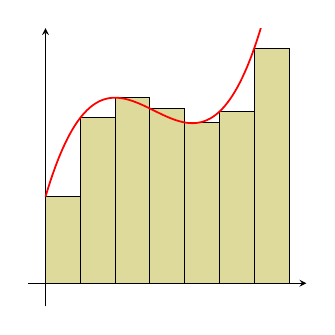
\begin{tikzpicture}[scale=0.8]
        \begin{axis}[
            axis lines=middle,
            xtick=\empty,
            ytick=\empty,
            xmin=-0.5, xmax=7.5,
            ymin=-0.5, ymax=5.5,
            width=6cm, height=6cm
        ]
        \addplot[ybar interval, fill=olive!30, domain=0:7, samples=8] {0.1 * (x-2)^3- 1/3 * (x-2)^2 + 4};
        \addplot[domain=0:7, samples=100, color=red, thick] {0.1 * (x-2)^3- 1/3 * (x-2)^2 + 4};
        \end{axis}
    \end{tikzpicture}
    \hspace{1cm}
    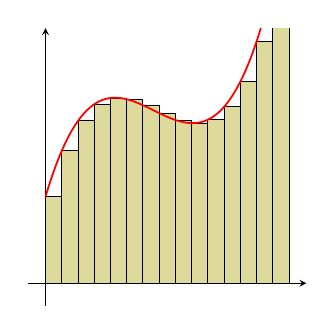
\begin{tikzpicture}[scale=0.8]
        \begin{axis}[
            axis lines=middle,
            xtick=\empty,
            ytick=\empty,
            xmin=-0.5, xmax=7.5,
            ymin=-0.5, ymax=5.5,
            width=6cm, height=6cm
        ]
        \addplot[ybar interval, fill=olive!30, domain=0:7, samples=16] {0.1 * (x-2)^3- 1/3 * (x-2)^2 + 4};
        \addplot[domain=0:7, samples=100, color=red, thick] {0.1 * (x-2)^3- 1/3 * (x-2)^2 + 4};
        \end{axis}
    \end{tikzpicture}
    \caption{Xấp xỉ diện tích bằng các hình chữ nhật.}
    \label{fig:rectangle_approx}
\end{figure}